\chapter{\label{c:speedmeter-intro}The \SSMEXPT{}: introduction and technical design}

\section{Position- and speed-meters}

\subsection{\label{sec:position-meter-measurement}Sensitivity of a position-meter}
In an ordinary \FPMI{} position-meter, the mirrors in each arm cavity are sampled by separate light beams which recombine at the beam splitter. Motion of each cavity in the longitudinal direction either shortens or elongates the round-trip phase of the light in each arm, and this motion is thus imprinted upon the \emph{phase} of the light returning to the beam splitter. The phase difference of the two recombining beams at the beam splitter then leads to light at the output port, which can be measured using a heterodyne or homodyne readout as discussed in Section\,\ref{sec:readout}.

The presence of classical light power in the arms leads to a radiation pressure effect which imparts a force upon the test masses. A restoring force on the mirrors, either via a pendulum in a suspended experiment or a mirror mount on a table-top experiment, means that this force is static and the interferometer can be held at the operating point as discussed in Section\,\ref{sec:operating-point} by microscopic \gls{DC} corrections.

\subsubsection{Input-output relations}
The signal that can be detected at the output port of a \FPMI{} can be calculated using \emph{input-output relations} defining the effect that some input signal would have on the output given the dynamics of the interferometer. In order to represent the effect that the interferometer has in terms of its effect on the amplitude and phase of the light, we use the \emph{two-photon formalism} \cite{Caves1985, Schumaker1985} which represents the input and output in terms of its \emph{cosine} and \emph{sine} quadratures, namely:
\begin{align}
  \vec{a} &=
  \begin{pmatrix}
    a_c \\
    a_s
  \end{pmatrix} \\
  \vec{b} &=
  \begin{pmatrix}
    b_c \\
    b_s
  \end{pmatrix},
\end{align}
where $\vec{a}$ is the input field and $\vec{b}$ is the output field. The output for an interferometer held at the dark fringe can be expressed as \cite{Danilishin2015}:
\begin{equation}
  \label{eq:ifo-output-signal}
  \vec{b} = \vec{R} \frac{h}{h_{\text{SQL}}} + \mathbb{T} \vec{a},
\end{equation}
where $\vec{R}$ is the response of the interferometer from unit mirror motion to the output, $\frac{h}{h_{\text{SQL}}}$ is the motion of the mirrors in terms of strain normalised to the \gls{SQL} as discussed in Section\,\ref{sec:sql} and $\mathbb{T}$ represents the transfer function of the input field to the output field.

The response $\vec{R}$ contains the effect that the mirror dynamics have on the readout, governed by the \emph{optomechanical coupling factor} $\kappa_{\text{MI}}$ defined for a \MI{} in Equation\,\ref{eq:optomechanicalcoupling}. This models the effect that an applied force to the mirror has on its position. Mirrors suspended from pendulum systems can be approximated at high frequencies to be a free mass, where the effect on position that an applied force has is diminished proportional to frequency, and in the case of a \FPMI{} this filtering effect scales as $\frac{1}{f^2}$ below the cavity's pole frequency, and $\frac{1}{f^4}$ above it.

The response to differential arm cavity motion, where the gravitational wave signal would appear, is given as:
\begin{equation}
  \label{eq:fp-mich-response}
  \vec{R}_{\left( - \right)} = \text{e}^{\text{i} \beta_{\text{FP}} \left( f \right)} \sqrt{2 \kappa_{\text{MI}}} \vec{H},
\end{equation}
where $\beta_{\text{FP}} \left( f \right)$ is the round-trip phase of the light in the arms and $\vec{H}$ represents the readout angle or \emph{quadrature}, $\zeta$:
\begin{equation}
  \vec{H} =
  \begin{pmatrix}
    \cos \zeta \\
    \sin \zeta
  \end{pmatrix}.
\end{equation}
The round-trip phase is defined:
\begin{equation}
  \beta_{\text{FP}} \left( f \right) = \arctan{\frac{f}{\gamma_{\text{arm}}}},
\end{equation}
where $\gamma_{\text{arm}}$ is the \FP{} cavity half-bandwidth (see Appendix\,\ref{sec:cavity-fom}).

In the case of \gls{DC} readout, as discussed in Section\,\ref{sec:homodyne-readout} and used in current generation detectors, the readout angle $\zeta = \SI{90}{\degree}$ represents the phase quadrature:
\begin{equation}
  \vec{H} =
  \begin{pmatrix}
    0 \\
    1
  \end{pmatrix}.
\end{equation}

We can calculate the signal at the \gls{DC} readout of the \FPMI{}, $O$, as a function of differential arm cavity motion by rearranging Equation\,\ref{eq:ifo-output-signal}:
\begin{equation}
  \frac{O_{\text{dc}} \left( f \right)}{h_{\left( - \right)}} = \frac{\text{e}^{\text{i} \beta_{\text{FP}} \left( f \right)} \sqrt{2 \kappa_{\text{MI}}}}{h_{\text{SQL}}}.
\end{equation}
This is shown in Figure\,\ref{fig:fp-mich-response} for arm length \SI{1}{\kilo\meter}, mirror mass \SI{40}{\kilo\gram}, laser wavelength \SI{1064}{\nano\meter} and cavity half-bandwidth \SI{200}{\hertz}. The units of magnitude are photons \SI{}{\per\sqrthz} strain.

\begin{figure}
  \centering
  \includegraphics[width=\columnwidth]{graphics/generated/from-python/40-fp-mich-response.pdf}
  \caption[Response of a \FPMI{} to differential arm cavity motion]{\label{fig:fp-mich-response}Response of a \FPMI{} to differential arm cavity motion. This shows the signal that would appear at a photodetector placed at the output of the interferometer given unit differential motion of the cavity. The cavity provides a signal with the same response for motion at frequencies below the cavity's pole frequency. Beyond the pole, the response is reduced as the motion becomes faster than the cavity's storage time.}
\end{figure}

The term $\mathbb{T}$ can be further broken down:
\begin{equation}
  \mathbb{T} = \text{e}^{2 \text{i} \beta_{\text{FP}} \left( f \right)}
  \begin{pmatrix}
    1 & 0 \\
    -\kappa_{\text{MI}} & 1
  \end{pmatrix},
\end{equation}
and so the optomechanical coupling factor transforms the input $\vec{a}$ in the sine quadrature by the mirror dynamics on its way to the output. The spectral density at the output port, $S \left( f \right)$, can be calculated as:
\begin{equation}
  S \left( f \right) = \left< \vec{b} \cdot \vec{b}^{\dag} \right>,
\end{equation}
and since the signal $h$ in the case of quantum noise is \num{0} we can define the output quantum noise $N \left( f \right)$:
\begin{equation}
  N \left( f \right) =
  \begin{pmatrix}
    1 & 0 \\
    -\kappa_{\text{MI}} & 1
  \end{pmatrix}
  \begin{pmatrix}
    a_c \\
    a_s
  \end{pmatrix}
  \begin{pmatrix}
    1 & -\kappa_{\text{MI}} \\
    0 & 1
  \end{pmatrix}.
\end{equation}

\subsubsection{Sensitivity of a \FPMI{}}
From the above definitions we can calculate the noise spectral density due to vacuum fluctuations at the output. Normal, unsqueezed vacuum has equal noise contributions in the cosine and sine quadratures, and so we can set it to the identity matrix:
\begin{equation}
  \label{eq:unsqueezed-vacuum-amplitude}
  \vec{a}_{\text{vacuum}} =
  \begin{pmatrix}
   1 & 0 \\
   0 & 1
  \end{pmatrix}.
\end{equation}
The quantum noise power spectral density is then:
\begin{equation}
  \begin{split}
    N \left( f \right) &=
    \begin{pmatrix}
      1 & 0 \\
      -\kappa_{\text{MI}} & 1
    \end{pmatrix}
    \begin{pmatrix}
      1 & 0 \\
      0 & 1
    \end{pmatrix}
    \begin{pmatrix}
      1 & -\kappa_{\text{MI}} \\
      0 & 1
    \end{pmatrix} \\
    &=
    \begin{pmatrix}
      1 & -\kappa_{\text{MI}} \\
      -\kappa_{\text{MI}} & 1 + \kappa^2_{\text{MI}}
    \end{pmatrix},
  \end{split}
\end{equation}
and the signal read by the \gls{DC} readout is then:
\begin{equation}
  \begin{split}
    N_O \left( f \right) &= \vec{H}^{T} N \left( f \right) \vec{H}
  \end{split}
\end{equation}

For \gls{DC} readout, the output noise spectral density is shown in Figure\,\ref{fig:fp-mich-noise}. This is the combination of radiation pressure noise from the mirrors and shot noise on the sensor, and these two effects combine to produce the quantum noise spectral density. At high frequencies, the quantum noise is equal to the quantum vacuum noise input from Equation\,\ref{eq:unsqueezed-vacuum-amplitude} (corresponding to $\kappa_{\text{MI}} \approx 0$) which shows that the signal on the sensor is limited by noise propagating to the output with no significant optomechanical interaction. Below the cavity pole, the vacuum fluctuations \checkme{move the mirror by an amount governed by the mirror's optomechanical coupling and so convert coherent cavity light into radiation pressure noise.}

\begin{figure}
  \centering
  \includegraphics[width=\columnwidth]{graphics/generated/from-python/40-fp-mich-noise.pdf}
  \caption[Quantum noise of a \FPMI{} at the output port]{\label{fig:fp-mich-noise}Quantum noise of a \FPMI{} at the output port. This shows the noise present at the photodetector produced due to quantum noise entering the interferometer and interacting with the mechanics. At high frequencies, the noise in a \MI{} is almost entirely due to the quantum shot noise on the sensor; at low frequencies the noise is dominated by the \checkme{light reaching the sensor due to fluctuations in the positions of the test masses due to quantum radiation pressure noise}.}
\end{figure}

The spectral density of the interferometer's sensitivity to differential arm cavity motion, $S_{\text{QNLS}}$, is given by the ratio of the quantum noise amplitude spectral density at the sensor to the response of the interferometer to that sensor for differential arm cavity motion, i.e.:
\begin{equation}
  S_{\text{QNLS}} = \frac{N_O}{O_{\text{dc}}} h_{\left( - \right)};
\end{equation}
this is shown in Figure\,\ref{fig:fp-mich-sensitivity}.

\begin{figure}
  \centering
  \includegraphics[width=\columnwidth]{graphics/generated/from-python/40-fp-mich-sensitivity.pdf}
  \caption[Sensitivity of a \FPMI{} at the output port to differential arm cavity motion]{\label{fig:fp-mich-sensitivity}Quantum noise limited sensitivity of a \FPMI{} at the output port to differential arm cavity motion. This is calculated by taking the quantum noise at the probe shown in Figure\,\ref{fig:fp-mich-noise} and dividing it by the response from differential arm cavity motion to the probe shown in Figure\,\ref{fig:fp-mich-response}. In this case the cavity power was chosen to touch the \gls{SQL} at the cavity pole and this is shown in the figure. For smaller cavity power, the touching frequency moves down.}
\end{figure}

\subsection{\label{sec:speed-meter-measurement}Sensitivity of a \SM{}}
Since the early 1990s it has been known that the measurement of momentum, known to be a quantum non-demolition (\gls{QND}) observable, offers the ability to surpass the \gls{SQL} in interferometric measurement \cite{Braginsky1990}. The force applied to test masses by a scheme involving the measurement of momentum does not affect its future value and so momentum can in principle be measured to arbitrary precision. Velocity is an appropriate observable to measure momentum and also approximates a \gls{QND} scheme due to its relation to momentum\footnote{Strictly, velocity is a \gls{QND} observable if the measurement is being made of a free mass \cite{Danilishin2012}. Since the test masses in a suspended interferometer are not free, this is only approximately correct in the frequency band far away from the suspension poles.}. Interferometers that measure velocity are called \emph{\SM{}s}. The principle of operation is as follows. The light from a laser enters the interferometer as it would for a position-meter, and accumulates a phase shift proportional to the propagation and the signal from any gravitational waves or disturbances in the positions of the mirrors. As the light reflects from the test masses within the interferometer it imparts radiation pressure from its light power and the quantum vacuum fluctuations as discussed in Section\,\ref{sec:position-meter-measurement}. Somewhere within the interferometer there must be mechanisms to impart a phase shift equivalent to \SI{180}{\degree} upon the light, and for it to then interact with the same test masses as it did before. Upon propagating through the interferometer a second time, the effect of the radiation pressure from the first pass is suppressed by the opposite sign of the radiation pressure from the second pass. This process is repeated many times due to the finesse of the cavities within the interferometer, though some light escapes to the output where it can be sensed. The cancellation of radiation pressure induced noise in a \SM{} type interferometer is a key benefit for gravitational wave detection.

The \SSM{} topology is being considered as an alternative to the proposed \MI{}s in the \ET{} \cite{MuellerEbhardt2009a, Voronchev2015}, though it represents only one of many different speed-meter topologies \cite{Danilishin2004, Wang2013, Huttner2016, Wade2012}. We consider here two of the most well known types to highlight the significantly different forms in which a \SM{} interferometer can take.

\subsubsection{The Michelson-type \SM{}}
Initial suggestions for the design of \SM{} type interferometers were focused on Michelson-like topologies, for instance with the addition of a \emph{sloshing cavity} \cite{Braginsky2000, Purdue2002} at the output port of a standard \FPMI{}, as shown in Figure\,\ref{fig:sloshing-michelson}. Here, the phase shift is imparted to the light by the addition of a beam splitter and cavity at the output of the interferometer. The light returning from the additional cavity is either re-injected into the interferometer or transmits through the beam splitter where it reflects from a signal recycling mirror. The light at the output of this interferometer then contains reduced quantum radiation pressure noise.

\begin{figure}
  \centering
  \includegraphics[width=\columnwidth]{graphics/generated/from-svg/40-sloshing-michelson.pdf}
  \caption[Layout of a \MI{} with a sloshing cavity]{\label{fig:sloshing-michelson}Layout of a \MI{} with a sloshing cavity as presented in \cite{Purdue2002}. The light leaving the standard \MI{} is coupled into a sloshing cavity via a beam splitter where it receives a phase shift, and it re-enters the interferometer via the recycling mirror to the left of the sloshing beam splitter. The light incident upon the beam splitter then contains light that has sampled the mirrors at two points in time, leading to a \SM{} effect.}
\end{figure}

\subsubsection{The Sagnac-type \SM{}}
It was later realised by Chen that the \emph{zero-area Sagnac} is a \SM{} \cite{Chen2003}. This topology is arranged such that incident photons enter into two counter-propagating modes which sample the position of the test masses at different intervals. The Sagnac interferometer was originally developed to measure the rotation of the Earth. To avoid this, the propagation of the light is arranged in this zero-area configuration to cancel this effect. Instead, the interferometer's output contains information of the difference in round-trip phase of the two counter-propagating modes. Given two test masses $A$ and $B$, over a time interval of $\Delta t$ each mode $A$ and $B$ will measure phase change arising from motion of the arms smaller than the light propagation time \cite{Chen2003}:
\begin{align}
  \delta \phi_{A} &\propto \Delta x_{A} \left( t \right) + \Delta x_{B} \left( t + \Delta t \right) \\
  \delta \phi_{B} &\propto \Delta x_{B} \left( t \right) + \Delta x_{A} \left( t + \Delta t \right),
\end{align}
where $\Delta x_{A}$ and $\Delta x_{B}$ are the differences in position of test masses $A$ and $B$, respectively. At the output port, the combined signal will then be:
\begin{equation}
  \begin{split}
    \delta \phi_{A} - \delta \phi_{B} &\propto \left( \Delta x_{A} \left( t \right) - \Delta x_{A} \left( t + \Delta t \right) \right) - \left( \Delta x_{B} \left( t \right) - \Delta x_{B} \left( t + \Delta t \right) \right) \\
                                      &\propto \Delta \dot{x}_{A} \left( t \right) - \Delta \dot{x}_{B} \left( t \right),
  \end{split}
\end{equation}
which shows that the signal is proportional to the relative velocity of the test masses. The output port is automatically at the dark fringe for the carrier light as long as the motion of the test masses is slower than the light propagation time. The output is not dark for the signal sidebands, and as they contain components from the test masses sampled at different times the signal is proportional to test mass speed.

The layout of a \SSM{} interferometer can be arranged in different forms, and we show one based on a zero-area Sagnac enhanced with ring cavities as arms in Figure\,\ref{fig:zero-area-ssm}.

\begin{figure}
  \centering
  \includegraphics[width=\columnwidth]{graphics/generated/from-svg/40-zero-area-ssm.pdf}
  \caption[Layout of a zero-area \SSM{}]{\label{fig:zero-area-ssm}Layout of a zero-area \SSM{}. The input light is split at the beam splitter where it forms two counter-propagating modes within the inner Sagnac mirrors. At each \gls{ITM}, the light is partially transmitted into the arm cavities, and upon exiting the cavities this light is sent either back to the beam splitter or to the next cavity. The recombined light at the beam splitter contains fields that have interacted with the position of all of the mirrors on its round trip and the difference in phase between the counter-propagating modes provides a signal proportional to relative test mass velocity.}
\end{figure} 

\subsubsection{Input-output relations}
The same approach to that for a \FPMI{} in Section\,\ref{sec:position-meter-measurement} can be taken to calculate the response and noise of a \SM{}, but with a value of $\kappa$ modified for a speed-meter \cite{Chen2003}:
\begin{equation}
  \kappa_{\text{SSM}} = 4 \kappa_{\text{MI}} \sin^2 \beta_{\text{FP}}.
\end{equation}
and as the round-trip phase includes both arms and an extra reflection from or transmission through the beam splitter, it is also modified:
\begin{equation}
  \beta_{\text{SSM}} = 2 \beta_{\text{FP}} + \frac{\pi}{2}.
\end{equation}

The response of a \SSM{} to differential arm cavity motion is shown in Figure\,\ref{fig:ssm-response}. Notice that below the cavity pole, the response vanishes towards \gls{DC}, consistent with a speed measurement. The higher response above the cavity pole is a consequence of the fact that the light samples the interferometer in both directions. For fair comparisons to the \MI{} the choice may be made to half the input power or change the readout angle.

\begin{figure}
  \centering
  \includegraphics[width=\columnwidth]{graphics/generated/from-python/40-ssm-response.pdf}
  \caption[Response of a \SSM{} to differential arm cavity motion]{\label{fig:ssm-response}Response of a \SSM{} to differential arm cavity motion. In contrast to the \MI{}, the \SSM{} has response proportional to frequency below the cavity pole.}
\end{figure}

The quantum noise at the output port is shown in Figure\,\ref{fig:ssm-noise}. Note that the noise is unity at high frequencies as with the \FPMI{}, but is suppressed at low frequencies due to the cancellation of back-action due to radiation pressure from quantum vacuum fluctuations.

\begin{figure}
  \centering
  \includegraphics[width=\columnwidth]{graphics/generated/from-python/40-ssm-noise.pdf}
  \caption[Quantum noise of a \SSM{} at the output port]{\label{fig:ssm-noise}Quantum noise of a \SSM{} at the output port. Like the \MI{}, the high frequency noise contribution arises from quantum shot noise from incoherent vacuum fluctuations entering the interferometer. In contrast to the \MI{}, the \SSM{} has flat noise at low frequencies below a transition region, as the test mass noise fluctuations are cancelled by the counter-propagating modes in the instance where the quantum radiation pressure forces are balanced.}
\end{figure}

While the response in a \SSM{} is reduced at low frequencies, the quantum noise is further reduced. Overall, the quantum noise limited sensitivity is improved in a \SSM{} over an equivalent \FPMI{} in the absence of loss, as shown in Figure\,\ref{fig:ssm-sensitivity}.

\begin{figure}
  \centering
  \includegraphics[width=\columnwidth]{graphics/generated/from-python/40-ssm-sensitivity.pdf}
  \caption[Sensitivity of a \SSM{} at the output port to differential arm cavity motion]{\label{fig:ssm-sensitivity}Quantum noise limited sensitivity of a \SSM{} at the output port to differential arm cavity motion. In contrast to the \MI{}, the \SSM{} sensitivity at low frequencies follows the gradient of the \gls{SQL} due to its reduced quantum noise. This improved sensitivity is in practice difficult to achieve as the presence of loss in the interferometer introduces a \emph{Michelson-like} sensitivity slope at a frequency proportional to the level of loss.}
\end{figure}

\subsubsection{Loss in \SSM{}s}
The \gls{QND} behaviour of the interferometer arises from the fact that the output port contains only commutative time-dependent momentum information. Time-\emph{independent} position information can, however, enter the output port of the interferometer in the presence of certain types of loss \cite{Danilishin2004}. For \emph{symmetric} loss, such as from imperfect transmissivity of the \glspl{ETM} or balanced substrate absorption in the \glspl{ITM}, a \emph{Michelson-like} sensitivity is introduced at a frequency proportional to the loss. Later it was shown that \emph{asymmetric} loss results in a greater decrease in sensitivity \cite{Danilishin2015}, with effects from imperfect beam splitting and imbalanced \gls{ITM} reflectivity considered.

The degradation in the sensitivity of a \SSM{} due to loss arises from the entry of vacuum fluctuations through the open ports created by loss mechanisms and from factors which result in imperfect cancellation of quantum radiation pressure effects. The optic most susceptible to asymmetries is typically the beam splitter, where coatings cannot be manufactured with better than around \SI{0.1}{\percent} tolerance\footnote{It turns out that the \SSM{} offers an excellent means of measuring a beam splitter's asymmetry.}. Imperfect splitting leads to different power in the counter-propagating modes which leads to optomechanical effects. In the \SSM{} this leads to light that would otherwise have exited at the input port of the interferometer instead exiting at the output port, carrying time-independent signal and therefore damaging the sensitivity. A similar effect arises from imbalances in the transmissivity of optics. This appears on sensitivity curves as an additional $\frac{1}{f}$ slope at low frequencies, like the position-meter behaviour shown in Figure\,\ref{fig:ssm-sensitivity}. The minimisation of loss is therefore critical in the design of a \SSM{} experiment.

\section{The Glasgow \SSMEXPT{}}
The Sagnac interferometer has been demonstrated in table-top experiments \cite{Shaddock1998} as well as lab-scale prototypes \cite{Beyersdorf2002} including the \gls{QND} behaviour of the \SSM{} \cite{Eberle2010} but so far this has not been demonstrated in a suspended prototype in the audio band to demonstrate its applicability for ground-based gravitational wave detectors. Here we present a proof-of-principle experiment in Glasgow to test audio-band reduction of quantum radiation pressure noise in a suspended \SSM{} over an equivalent Michelson design \cite{Graef2014}. The \SSM{} is enhanced with the presence of triangular ring cavities to enhance the sensitivity of the interferometer to differential motion of the arms, and balanced homodyne readout will be utilised to sense the quantum correlations present at the otherwise dark output.

Quantum radiation pressure noise depends inversely upon the reduced mass of the arm cavities. In order for the interferometer to be dominated by quantum radiation pressure noise at low frequencies, one of the \emph{core} optics in each of the triangular arm cavities will be much lighter than the other two to facilitate a reduced mass of around \checkme{\SI{0.8}{\gram}}. The \glspl{ETM} in this case will be around \SI{100}{\gram} while the \glspl{ITM} will be around \SI{1}{\gram}. As the intracavity power will be around \checkme{\SI{4}{\kilo\watt}}, the radiation induced force will be significant enough to measure above other noise sources at frequencies between \num{100} and \SI{700}{\hertz}.

The intended optical layout is shown in Figure\,\ref{fig:ssm-layout}. The light is coupled by the main beam splitter \MSIX{} into counter-propagating modes in the \emph{inner Sagnac}, i.e. the cavity formed by the mirrors \MSIX{}, \MSEVEN{}, \MONEA{}, \MTEN{}, \MNINE{}, \MEIGHT{} and \MONEB{}. At \glspl{ITM} \MONEA{} and \MONEB{} the light is partially transmitted into arm cavities $A$ and $B$, respectively, where the light is resonantly enhanced by the highly reflective \glspl{ETM} \MTWOA{} and \MTHREEA{} and \MTWOB{} and \MTHREEB{}. Upon exiting the cavities, the light again propagates through the inner Sagnac where it recombines at \MSIX{}. The light leaving \MSIX{} towards \MFOURTEEN{} contains the signal encoded as quantum correlations on the light, and this is enhanced at \MSIXTEEN{} by the local oscillator provided by the light leaving \MSIX{} towards \MTWELVE{}. The balanced homodyne detectors (\gls{BHD}) \HDA{} and \HDB{} measure the transmitted light, and the difference signal primarily contains information regarding the relative velocity of the arm cavities.

\begin{figure}
  \centering
  \includegraphics[width=\columnwidth]{graphics/generated/from-svg/40-speedmeter-layout.pdf}
  \caption[\SSMEXPT{} layout]{\label{fig:ssm-layout}\SSMEXPT{} layout. The in-vacuum part of the experiment will be situated in two \SI{1}{\meter} diameter tanks joined with a connecting tube. The suspended optics will be placed on breadboards atop passive isolation stacks, joined together with a bridge structure. Viewports are situated on both tanks at each side to facilitate in-air sensing. The vacuum system is capable of reaching pressures below \SI{e-6}{\milli\bar} to suppress the impact of residual gas noise.}
\end{figure}

The interferometer is to be situated within an ultra-high vacuum system formed from two adjoined cylindrical tanks with pumps capable of reaching pressures of \SI{1e-6}{\milli\bar}. Each tank contains a breadboard for the attachment of components, and this breadboard is itself isolated from ground motion by a series of passive damping stacks. The breadboards are rigidly connected via a bridge structure to ensure that residual platform motion is common to all suspended optics. The optics will be suspended from pendulum systems, with the most important test masses suspended from multiple stages to provide additional isolation from seismic noise. The parameters for the optics, laser injection, suspension systems and materials can be found in \cite{Graef2014}, \cite{Danilishin2015} and \cite{Leavey2016} in chronological order.

\subsection{\label{sec:bhd-intro}Balanced homodyne detection}
\note{Explain homodyne angle, basic description.}
The readout mechanism for the gravitational wave channel, the differential arm cavity degree of freedom, will be balanced homodyne readout. This choice contrasts to the \emph{de-facto} standard in gravitational wave observatories, \gls{DC} readout, because it is necessary for the measurement of sensitivity below the \gls{SQL} in the presence of imprecisely known loss to be able to alter the homodyne angle of the readout. In \gls{DC} readout, the homodyne angle is fixed by the propagation length between the detuned arm cavities and the output port. Balanced homodyne readout can choose arbitrary homodyne angles through the tuning of the relative phase of the (separate) local oscillator and signal paths.

Balanced homodyne readout involves making a subtraction of two signals measured in this case by \HDA{} and \HDB{}, observing light combined from a local oscillator, $a$, and the signal output of the \SSM{}, $b$. The local oscillator field should not contain signal, and so this will be taken from the light reflected from the interferometer back towards the input, via \MTWELVE{} and \MTHIRTEEN{}. The signal power measured at each photodetector output $c$ and $d$ then contains \cite{Steinlechner2015}:
\begin{equation}
  \begin{split}
    c^{\dag} c &= \frac{1}{2} \left( a^{\dag} a + a^{\dag} b \text{e}^{-\text{i} \phi} + a b^{\dag} \text{e}^{\text{i} \phi} + b^{\dag} b \right) \\
    d^{\dag} d &= \frac{1}{2} \left( a^{\dag} a + a^{\dag} b \text{e}^{\text{i} \phi} + a b^{\dag} \text{e}^{-\text{i} \phi} + b^{\dag} b \right),
  \end{split}
\end{equation}
where $\phi$ is the homodyne angle. The mixing of the two signals at \MSIXTEEN{} results in the \gls{DC} part of one field beating with the \gls{AC} part of the other field, and so a delicate subtraction of the two photocurrents from \HDA{} and \HDB{}, $I_{\text{BHD}}$, results in only the \gls{AC} parts corresponding to the motion of the test masses amplified by the local oscillator field:
\begin{equation}
  \begin{split}
    I_{\text{BHD}} &= c^{\dag} c - d^{\dag} d \\
                   &= a^{\dag} b \text{e}^{\text{i} \phi} - a^{\dag} b \text{e}^{\text{-i} \phi} + a b^{\dag} \text{e}^{\text{i} \phi} - a b^{\dag} \text{e}^{\text{-i} \phi}.
  \end{split}
\end{equation}
Laser noise and residual carrier light in the signal path can result in vastly increased noise in this readout scheme and so it is important for the relative intensity noise of the laser to be controlled to a high level and for the use of a beam splitter with balanced reflectivity and transmissivity \cite{Steinlechner2015}.

\subsection{Quantum noise limited sensitivity of the main readout}
Without including the effect of asymmetric loss, the quantum noise limited sensitivity of the \gls{BHD} readout in the \SSMEXPT{} calculated with both Finesse and Optickle (see Appendices \ref{sec:finesse-sim} and \ref{sec:optickle-sim}) is shown in Figure\,\ref{fig:erc-ssm-qnls}. Also shown is an equivalent \MI{} using the same parameters and mirrors as the \SSM{}, but with input power scaled by a factor of approximately \num{2.5} to match the high frequency sensitivities. The homodyne angles of the \SSM{} and \MI{} are \SI{45}{\degree} and \SI{90}{\degree}, respectively, fairly optimise both interferometers for high frequency sensitivity. The intended measurement band is between \SI{100}{\hertz} and \SI{700}{\hertz}, and so a reduction of a factor of around \num{3} to \num{5} is in theory possible as long as other sources of noise are sufficiently low. A full consideration of the noise budget is given in Chapter\,\ref{c:speedmeter-control}.
% Homodyne angles for SSM vs MI from https://arran.physics.gla.ac.uk/wp/speedmeter/?p=5648

\begin{figure}
  \centering
  \includegraphics[width=\columnwidth]{graphics/generated/from-python/40-erc-ssm-qnls.pdf}
  \caption[Quantum noise limited sensitivity of the \SSMEXPT{}]{\label{fig:erc-ssm-qnls}Quantum noise limited sensitivity of the \SSMEXPT{} calculated with Optickle and Finesse. Also shown is the equivalent \MI{} configuration, calculated with Optickle, and the \gls{SQL} given the effective mass of the interferometer test masses. The shaded \checkme{blue} region shows the intended measurement band, where reduced quantum radiation pressure noise should be visible below the expected noise from the equivalent \MI{}.}
\end{figure}

\subsection{Sensing and control}
The main readout of the \SSMEXPT{} is to be the \gls{BHD} at the output port, however in order to control the interferometer a number of other signals will need to be extracted and fed back to actuators to keep the interferometer at the operating point, as described in Section\,\ref{sec:operating-point}. This can be split into two broad categories representing the process used to bring the interferometer to the operating point, \emph{lock acquisition}, and keeping it there, \emph{low-noise} control.

The interferometer's test masses will drift from the operating point due to the noise imparted from quantum, seismic, thermal and other noise sources as discussed in Section\,\ref{sec:ifo-foundations} if they are not actively controlled. This control takes the form of longitudinal and angular actuators at each test mass and feedback to the main laser's temperature and frequency. In the \SSMEXPT{} there are a few major control topics that must be solved in order to reach the required sensitivity:
\begin{enumerate}
  \item The control of longitudinal drifts in the positions of the test masses, which leads to loss of cavity power and sensitivity;
  \item The control of angular drifts in the optics, particularly from the triangular arm cavities and especially important for the small \glspl{ITM} where radiation pressure effects will be significant;
  \item The control of intensity noise on the main laser.
\end{enumerate}
The first two topics are tackled through the identification of the degrees of freedom of the interferometer and the selection of appropriate readout ports. The last involves the implementation of an appropriate frequency stabilisation control servo.

The process of bringing the interferometer to its operating point is challenging in interferometers with multiple degrees of freedom and typically requires modelling of the interferometer in the time domain to understand the effect that changes to actuator feedback signals, radiation pressure effects and noise couplings have on the system. In the case of the \SSMEXPT{} this is particularly challenging due to the coupling between the arm cavities from the counter-propagating modes. A lock acquisition model has been developed which should in principle be able to deterministically bring the interferometer to the operating point \cite{Glaefke2015}.

\subsubsection{\label{sec:cds}Data acquisition and software control}
The control and data acquisition system developed for \gls{LIGO}, \emph{\gls{CDS}} \cite{Bork2010}, is appropriate for the \SSMEXPT{} and a great deal of effort has already gone in to making this system useful and reliable for the control of complicated experiments. This system takes the form of many \emph{off-the-shelf} components and some custom software to provide the ability to sense and feedback control signals at speeds of up to around \SI{10}{\kilo\hertz}. Extensive software is also available for offline data analysis.

The translation between the digital \gls{CDS} domain and the analogue domain takes the form of analogue-to-digital and digital-to-analogue converters (\glspl{ADC} and \glspl{DAC}) situated on a \emph{front-end} computer which runs software control modules in real time. A \emph{frame builder} computer communicates with the front end(s) over a fast network in order to build packets of measurements in \gls{GPS}-synchronised intervals.

\subsection{Suspensions}
The \emph{auxiliary} optics \MFOUR{}, \MFIVE{}, \MSEVEN{}-\MTEN{} and \MTWELVE{}-\MFIFTEEN{} will be suspended from two stage pendulum systems. These steering optics do not have as stringent residual motion requirements as the test masses and so these suspensions can be relatively simple in design in comparison. The core optics will be suspended from two different systems: the \SI{100}{\gram} test masses from triple stage suspensions co-designed for the \SSMEXPT{} and the \AEIPROTOTYPE{}, and the \SI{1}{\gram} test masses from bespoke \checkme{triple stage} suspensions. The beam splitter \MSIX{} will require one additional design loosely based on the auxiliary suspensions. Each optic class requires a separate suspension design due to the differences in geometry and the need to move the mechanical modes from each of the suspensions' degrees of freedom out of the measurement band.

\subsection{Actuation}
The auxiliary suspensions will have voice coil actuators on their intermediate stages for initial alignment control. Each of the \glspl{ETM} will have voice coils on multiple stages in order to provide corrections for low frequency drifts. The test mass stages will not have voice coil actuators to minimise the prevalence of \emph{Barkhausen} \cite{Weiss2008} and electronic noise coupling to the positions of the test masses via the actuators' magnets and driver electronics. The filtering effect from the final pendulum stage means that the voice coil actuators will not be able to effectively correct positions at high frequencies. Instead, \emph{electrostatic drive} (\gls{ESD}) actuators will be placed behind each \gls{ETM} able to produce small corrective forces but with expected lower noise than equivalent voice coils. \gls{ESD} actuators have been demonstrated in \GEO{} \cite{Hewitson2007} and \ALIGO{} \cite{Aston2012} based on a metallic comb arrangement, however in the \SSMEXPT{} the intention is to use a new \gls{ESD} design.

% you know what? why the hell would anyone care about this section?
% \subsubsection{Coil drivers}
% The coil drivers for the auxiliary suspensions have been designed with a simple two-pole low-pass filter circuit. As there will be at least \num{14} suspensions requiring auxiliary coil drivers, some thought has been dedicated to the signalling from \gls{CDS} to the experiment.
% 
% Each \gls{CDS} output connector contains four channels and each auxiliary suspension has four coils, so each coil driver supports a single suspension with a single input from \gls{CDS}. These coil drivers are build on Eurocard format printed circuit boards (\glspl{PCB}) with DIN \num{41612} connectors. These cards slot into a custom-built backplane board housed within a standard \checkme{3 height-unit} rack enclosure. On the rear of this enclosure are two 50-way DSUB connectors capable of carrying the signals for up to \num{7} auxiliary coil drivers each.
% 
% \note{Put aux coil driver stuff here}
% \note{Auxiliary coil driver subrack wiring design / motivation / assembly}
% \note{Backplane board design - talk about rationale, show Eagle diagrams, etc.}
% 
% \begin{figure}
%   \centering
%   \includegraphics[width=\columnwidth]{graphics/generated/from-svg/40-auxiliary-octopus-cable.pdf}
%   \caption[Auxiliary octopus cable schematic]{\label{fig:aux-octopus-cable-wiring}``Octopus'' cable for breaking out a DB50 connector into DB9 connectors to allow signals to be sent to each of the coils on seven auxiliary suspensions.}
% \end{figure}
% 
% \begin{figure}
%   \centering
%   \includegraphics[width=\columnwidth]{graphics/generated/from-svg/40-auxiliary-suspension.pdf}
%   \caption[Auxiliary suspension coil schematic]{\label{fig:aux-suspension-wiring}Auxiliary suspension coil schematic.}
% \end{figure}
% 
% \begin{figure}
%   \centering
%   \includegraphics[width=\columnwidth]{graphics/generated/from-svg/40-auxiliary-backplane-board.pdf}
%   \caption[Auxiliary subrack backplane board schematic]{\label{fig:aux-backplane-schematic}Auxiliary coil driver subrack backplane. Auxiliary coil driver cards can be plugged in to this board, which then maps the signals to a DB50 connector which connects to the vacuum feedthrough. This routes four coil signals (five conductors including ground) per coil driver, for seven coil drivers, to one DB50 connector. This can then be connected to the vacuum system, where the auxiliary octopus cable (see Figure XXX) maps these signals to individual auxiliary suspensions.}
% \end{figure}
% 
% \begin{figure}
%   \centering
%   \includegraphics[width=\columnwidth]{graphics/generated/from-svg/40-auxiliary-backplane-interface.pdf}
%   \caption[Auxiliary subrack backplane interface]{\label{fig:aux-backplane-interface}Auxiliary coil driver subrack backplane interface.}
% \end{figure}

% or this one?
% \subsection{Signalling}
% 
% \subsubsection{In-vacuum}
% \note{Octopus cables, strain relief housing, etc.}
% 
% \begin{figure}
%   \centering
%   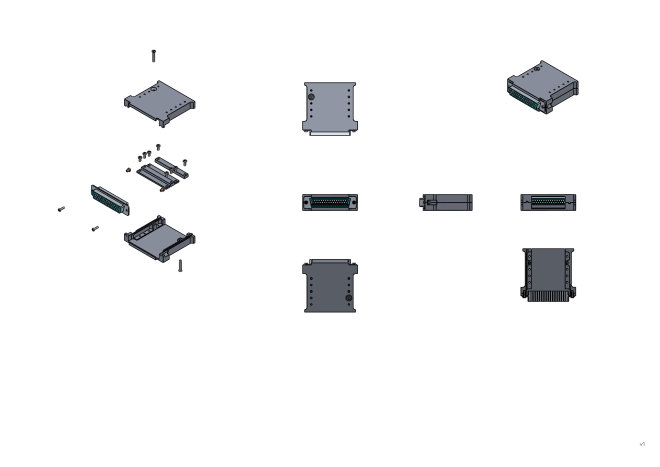
\includegraphics[width=0.75\columnwidth]{graphics/40-db50-housing.png}
%   \caption[In-vacuum DB50 octopus cable housing]{In-vacuum DB50 housing for octopus cable.}
%   \label{fig:db50-housing}
% \end{figure}

\section{Topics of particular focus}
There are many areas of research and development required in order to meet the challenging goals of the \SSMEXPT{}, but we will focus in particular on the strategy for controlling the longitudinal degrees of freedom of the interferometer at its operating point. Chapter\,\ref{c:speedmeter-control} will develop a sensing and control scheme for the interferometer taking into account anticipated sensors, actuators and noise sources. Chapter\,\ref{c:esd-concept} will present the design of the high voltage electronics and signalling for the \gls{ESD} design to be used in the experiment. A summary is provided in \note{conclusion chapter}.